\section{Design Techniques}
\blue{Techniques to implement} \red{design principles}
This lecture is about techniques to improve/establish
\begin{itemize}
    \item design and code \red{comprehensibility}
    \item \red{cohesion} by moving/reassigning responsibilities
\end{itemize}
In particular, we look at 
\begin{itemize}
    \item \red{Documentation}
    \item \red{Refactoring}
    \item \red{Design Patterns} 
\end{itemize}
\subsection{Part I: Documentation}
\subsubsection{Comprehensibility: Readability \& Documentation}
\begin{defBox}[title=Readability requires: ...]
    \begin{itemize}
        \item \red{Documentation} (explain design, architecture, ...relative to requirements)
        \item Source code \red{comments}:
        \begin{itemize}
            \item \red{API} documentation of each package, interface, class, method
            \item \red{Line} comments
        \end{itemize}
        \item Source \red{code}
    \end{itemize}
\end{defBox}
\begin{defBox}[title=Code Specific Aspects]
    \begin{itemize}
        \item Coding style \red{conventions} (on which line to write \{ ...)
        \item \red{Restrictions} on usage of language features (MISRA-C)
        \item Good \red{naming} of identifiers (classes, fields, methods, method parameters, local variables, etc.)
        \item Meaningful \red{comments}
    \end{itemize}
\end{defBox}
\subsubsection{Documentation: Commenting a Method Implementation}
\begin{defBox}
    How many lines of comment for method getImage()?
\end{defBox}
\clearpage
\subsubsection{Documentation: Example of a Java Source Code Comment}
\begin{figure}[h]
    \centering
    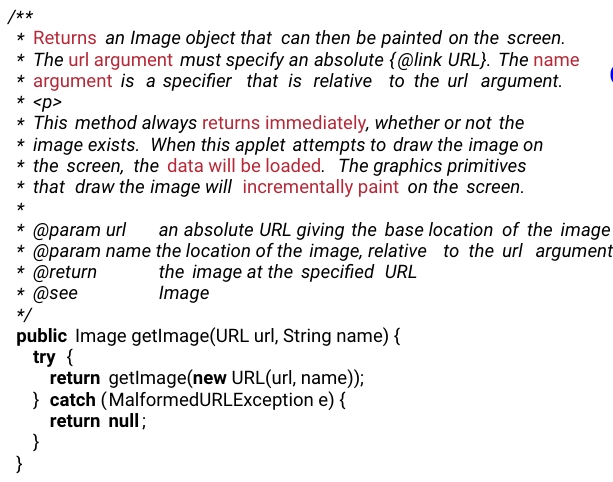
\includegraphics[width=1\textwidth]{Images/Example of a Java Source Code Comment.jpeg}
\end{figure}
\blue{Observations}
\begin{itemize}
    \item Length of source code vs. comment
    \item Comment adds \red{useful} information
    \begin{itemize}
        \item parameter format 
        \item behavior
        \item side effects
    \end{itemize}
    \item Comments rendered as HTML + keywords $\Rightarrow$ API documentation
\end{itemize}
\subsubsection{Documentation: Source Code Comments}
\blue{Two kinds of source code comments:}
\begin{itemize}
    \item (Public) \red{API} comment: class level and method level
    \item \red{Statement} level comments
\end{itemize}
\begin{defBox}[title=API comments]
    \red{Intent:} API usage documentation\\
    \red{Audience:} Third-party developers using the code as framework/library\\
    Describe in detail \red{when} method may be called and its \red{behavior}:
    \begin{itemize}
        \item Additional restrictions on parameters besides type (e.g., not null reference or non-negative)
        \item Side-effects on object state
        \item When and which exceptions are thrown
    \end{itemize}
\end{defBox}
\begin{infoBox}[title=API-Kommentare: Eine Übersicht]
    API-Kommentare dienen als Dokumentation für Drittentwickler, die eine Codebasis als Framework oder Bibliothek verwenden. Sie stellen sicher, dass Entwickler die Methoden korrekt nutzen und verstehen, welche Bedingungen erfüllt sein müssen und welche Auswirkungen die Methoden haben können.
\end{infoBox}
\begin{infoBox}[title=Ziel(Intent):]
    \begin{itemize}
        \item \fatsf{Dokumentation der Nutzung} der API für Entwickler
        \item Sicherstellen, dass Entwickler wissen, \fatsf{wann} und \fatsf{wie} eine Methode aufgerufen werden kann
    \end{itemize}
\end{infoBox}
\begin{infoBox}[title=Zielgruppe(Audience):]
    \begin{itemize}
        \item \fatsf{Drittentwickler}, die die API oder Bibliothek nutzen, aber keinen direkten Zugriff auf den internen Code haben
    \end{itemize}
\end{infoBox}
\begin{infoBox}[title=Wichtige Inhalte von API-Kommentaren:]
    \begin{enumerate}
        \item \fatsf{Wann eine Methode aufgerufen werden kann:}
        \begin{itemize}
            \item Kontext des Aufrufs(z.B. muss eine Verbindung hergestellt sein)
            \item Lebenszyklusbedingungen (z.B. nach Initialisierung, vor dem Schließen eines Objekts)
        \end{itemize}
        \item \fatsf{Verhalten der Methode:}
        \begin{itemize}
            \item Welche Aktion wird ausgeführt?
            \item Welche Änderungen treten auf?
        \end{itemize}
        \item \fatsf{Zusätzliche Einschränkungen für Parameter:}
        \begin{itemize}
            \item Anforderungen, die über den Datentyp hinausgehen:
            \begin{itemize}
                \item \fatsf{Nicht-null-Referenzen:} Der Parameter darf nicht null sein
                \item \fatsf{Wertebereiche:} Zahlenwerte müssen positiv oder in einem bestimmten Bereich sein
            \end{itemize}
        \end{itemize}
        \item \fatsf{Nebenwirkungen auf den Objektzustand:}
        \begin{itemize}
            \item Welche Felder oder Zustände des Objekts ändern sich nach dem Methodenaufruf?
        \end{itemize}
        \item \fatsf{Ausnahmen(Exceptions):}
        \begin{itemize}
            \item Wann und warum eine Methode eine Ausnahme auslöst
            \item Typen von Ausnahmen und deren Bedeutung
        \end{itemize}
    \end{enumerate}
\end{infoBox}
\begin{defBox}[title=Statement level comments]
    \red{Intent:} Describe implementation details, structure code\\
    \red{Audience:} Developers on the same code base\\
    Should be \red{concise} and used sparingly
    \begin{itemize}
        \item Clear and well-wirtten code is-to an extent-self-documenting
        \item Might be an indication of overly complex code\\
        $\Rightarrow$ \fatsf{Refactor!}
    \end{itemize}
\end{defBox}

\subsection{Part II: Refactoring}
\subsubsection{Refactoring: Definition}
\enquote{\red{Refactoring} is a disciplined technique for restructuring an existing body of code, altering its internal structure \blue{without changing its external behavior}}
\begin{defBox}[title=Objectives]
    \begin{itemize}
        \item \red{Preparing} addition of new features (\red{not} addition of new features)
        \item Improving design, for example, increasing \red{cohesion}
        \item Increasing \red{comprehensibility}
        \item Improving \red{maintainability} of the software
    \end{itemize}
\end{defBox}
\subsubsection{Refactoring: Reasons to Refacor Design and Code}
\begin{defBox}
    Assume we want to add a feature for querying cars with certain number of seats
\end{defBox}
\begin{codeBlock}{}
    public class Query{
        List<Car> cars;
        public List<Car> cars;
        public List<Car> getCarsOfModel(String model){
            List<Car> filteredCars = new LinkedList<>();
            for(Car c : cars){
                if(model.equals(c.getModel())){
                    filteredCars.add(c);
                }
            }
            return filteredCars;
        }
    }
\end{codeBlock}
\blue{Addition of New Features}\\
Restructureing makes \red{adding new feature easier:}
\begin{itemize}
    \item Less code duplication
    \item Avoid nested conditions, etc.
\end{itemize}
\begin{defBox}
    Quick and dirty: Copy \& Paste\\
    \blue{Disadvantages:}
    \begin{itemize}
        \item Code duplication
        \item No support for future extensions (other query types)
    \end{itemize}
\end{defBox}
\begin{codeBlock}{}
    public class Query{
        public List<Car> cars;
        public List<Car> getCarsOfModel(String model){...}
        public List<Car> getCarsWithSeats(int seats){
            List<Car> filteredCars = new LinkedList<>();
            for(Car c : cars){
                if(c.getSeats() == seats){
                    filteredCars.add(c);
                }
            }
            return filteredCars;
        }
    }
\end{codeBlock}
\begin{defBox}
    \red{Parameterize} method with property \red{f} to filter as a new argument\\
    Filtering for car properties now flexible:\\
    \blue{filterCars(Car::getModel, \enquote{Golf})}\\
    or\\
    \blue{filterCars(Car.:getSeats, 5)}
\end{defBox}
\begin{codeBlock}{}
    public class Query{
        List<Car> cars;
        public <T>List<Car> filterCars(Function<Car, T> f, T value){
            List<Car> filteredCars = new LinkedList<>();
            for(Car c : cars){
                if(value.equals(f.apply(c))){
                    filteredCars.add(c);
                }
            }
            return filteredCars;
        }
    }
\end{codeBlock}
\begin{figure}[h]
    \centering
    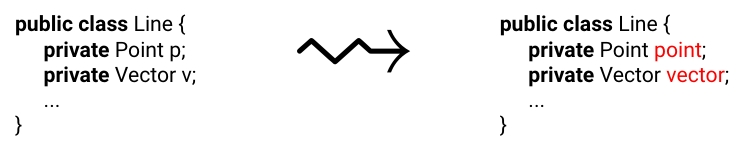
\includegraphics[width=0.75\textwidth]{Images/Reasons to Refactor Design and Code.jpeg}
\end{figure}
\blue{Comprehensibility}\\
Restrucuring makes design or code easier to understand:
\begin{itemize}
    \item Choose meaningful names for variables, methods, ...
    \item Simplify unnecessarily convoluted program logic
\end{itemize}
\clearpage
\subsubsection{Refactoring Techniques}
\subsubsection*{Example: A Statistics Class for CaSh}
\begin{figure}[h]
    \centering
    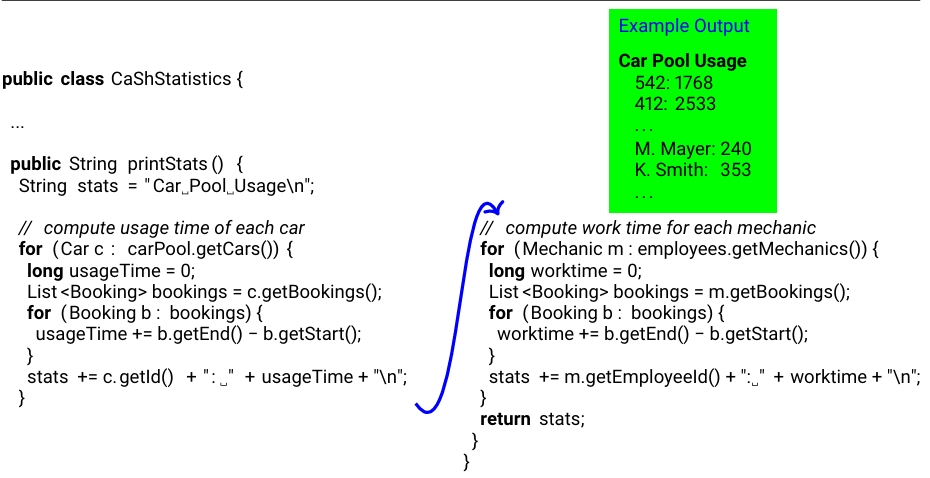
\includegraphics[width=1\textwidth]{Images/A Statistics Class for Cash.jpeg}
\end{figure}
\subsubsection*{Extract Method}
\begin{defBox}[title=When to Use?]
    \begin{itemize}
        \item One Method does several things (Computers usage time, work time and composes statistics)
        \item Similar functionality realized within one or as part of several methods
    \end{itemize}
\end{defBox}
\begin{defBox}[title=Extract Method]
    \begin{enumerate}
        \item Create new method (target)
        \item Copy extracted code to target
        \item Identify set of local variables used in extracted code
        \begin{enumerate}
            \item Variables only used in extracted code declared as local variables
            \item Exactly one local variable modified: check if target method can be query
            \item More than one local variable modified: Extract Method not applicable
            \item Pass undeclared local variables as method arguments
        \end{enumerate}
        \item Replace extracted code in refactoring source with call to extracted method
    \end{enumerate}
\end{defBox}
\begin{codeBlock}{}
    public class CaShStatistics{
        ...
        public String printStats(){
            String stats = "Car Pool Usage\n";
            //compute usage time of each car
            for (Car c : carPool.getCars()){
                long usageTime = computeCarUsageTime(c);
                stats += c.getId() + ": " + usageTime + "\n";
            }
            //compute work time for each mechanic
            ...
        }
        private long computeCarUsageTime(Car c){
            long usageTime = 0;
            List<Booking> bookings = c.getBookings();
            for (Booking b : bookings){
                usageTime += b.getEnd() - b.getStart();
            }
            return usageTime;
        }
    }
\end{codeBlock}
Applying \red{Extract Method} twice
\begin{defBox}[title=Observation 1]
    \blue{usageTime, worktime} only used \red{once}\\
    $\Rightarrow$ Apply refactoring \red{Inline Temp}
\end{defBox}
\begin{defBox}[title=Observation 2]
    Improve readability by extracting methods for printing usage time \& worktime \red{and} call usage methods from there
\end{defBox}
\begin{defBox}[title=Observation 3]
    Comments in printStats() do not add anything useful any more $\Rightarrow$ Remove
\end{defBox}
\begin{codeBlock}{}
    public class CaShStatistics{
        ...
        public String printStats(){
            String stats = "Car Pool Usage\n"
            stats = printCarUsageTime(stats);
            stats = printMecahnicsWorktime(stats);
            return stats;
        }
        private String printCarUsageTime(String s){...}
        private String printMecahnicsWorktime(String s){...}
        private long computeCarUsageTime(Car c){...}
        private long computeWorktime(Mechanic m){...}
    }
\end{codeBlock}
\subsubsection*{Move Method-Improving Cohesion}
\begin{codeBlock}{}
    public class CaShStatistics{
        ...
        private long computeCarUsageTime(Car c){
            long usageTime = 0;
            List<Booking> bookings = c.getBookings();
            for (Booking b : bookings){
                usageTime += b.getEnd() - b.getStart();
            }
            return usageTime;
        }
        private String printCarUsageTime(String s){...}
    }
\end{codeBlock}
\red{Cohesion got worse!}\\
computeCarUsageTime(), computeWorktime() do not use \red{fields} of class CaShStatistics (not even methods)\\
\blue{Make them static?} Not a good Solution in this case\\
\blue{Problem at the core:} \red{CaShStatistics has too many responsibilities}\\
Method computeCarUsageTime() \red{belongs actually to} Car (similarly computeworktime() to Mechanic)\\
$\Rightarrow$ Use refactoring \red{Move Method}
\begin{defBox}[title=Applicability Check for Move Method]
    Does the source method (here: \blue{computeCarUsageTime()})
    \begin{itemize}
        \item use features of the source class (here: CaShStatistics)?
        \item override a method or is overriden by a subclass?
    \end{itemize}
    If answer is no, then \red{Move Method} is applicable\\
    (otherwise other refactorings/preparation may first be necessary, see M. Fowler, \enquote{Refactoring})
\end{defBox}
\begin{defBox}[title=Applying Move Method]
    \begin{enumerate}
        \item \red{Declare} method in target class
        \item Copy source method to target class and \red{adjust} method to work there
        \item Determine how to reference target object from source (\red{delegation})
        \item Turn source method into \red{delegating} method
        \item Source method may be \red{removed} if not needed, also \red{accessors} in target class
    \end{enumerate}
\end{defBox}
\begin{codeBlock}{}
    public class CaShStatistics{
        ...
        private String printCarUsageTime(String s){
            for (Car c : carPool.getCars()){
                s += c.getId() + ": " + c.getUsageTime() + "\n";
            }
            return s;
        }
    }
    public class Car{
        ...
        public long getUsageTime(){
            long usageTime = 0;
            List<Booking> bookings = this.getBookings();
            for(Booking b : bookings){
                usageTime += b.getEnd() - b.getStart();
            }
            return usageTime;
        }
    }
\end{codeBlock}
\subsubsection*{Extract Class}
\begin{defBox}[title=Refactoring Extract Class]
    Apply \red{Extract Class}, if a class has two or more independent responsibilities and no other class is suitable to move the corresponding fields and methods\\
    Like \fatsf{Move Method}, improves cohesion, more generally applicable
\end{defBox}
\begin{defBox}[title=Applying Extract Class]
    \begin{enumerate}
        \item \red{Create} new class
        \item \red{Link} new class from old clas, may need new \red{accessor} method
        \item Apply refacotring \red{Move Field} (not shown)
        \item Apply refactoring \red{Move Method}
        \item Review and reduce class interfaces (unnecessary accessors ...)
    \end{enumerate}
\end{defBox}
\begin{figure}[h]
    \centering
    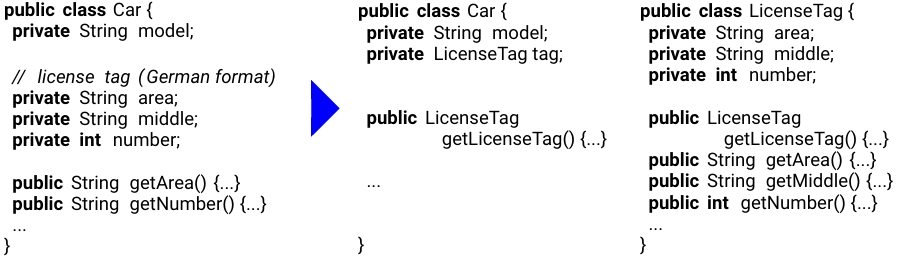
\includegraphics[width=1\textwidth]{Images/Extract Class.jpeg}
\end{figure}
\subsection{Part III: Design Patterns-Introduction}
\subsubsection{Design Patterns}
A \red{design pattern} describes ...
\begin{itemize}
    \item a \red{problem} that \red{reoccurs} regularly in our domain,
    \item is the core of a \red{solution} to that problem, such that one can reuse this solution many times, never in exactly the same way
\end{itemize}
\blue{Motivation}
\begin{itemize}
    \item Designing reusable software is \red{hard}
    \item Novices are \red{overwhelmed}
    \item Experts draw from \red{experience}
    \item Some design solutions \red{reoccur}
\end{itemize}
\blue{Understanding reoccuring solutions has different facets}
\begin{itemize}
    \item Know \red{when} to apply
    \item Know the \red{consequences} (trade-offs)
\end{itemize}
\subsubsection{Some Remarks on Software Patterns}
\begin{itemize}
    \item Software design patterns are part of the \red{current software practice}
    \begin{itemize}
        \item Used and implemented in APIs+documentation (Java Standard Library)
    \end{itemize}
    \item \red{Criticism:} Lack of scientific evaluation on effects of design patterns
    \begin{itemize}
        \item Some studies even indicate averse effects for certain patterns
        \item Further inverstigations of the underlying reasons necessary
    \end{itemize}
    \item Standard book: Erich Gamma et al., \red{Design Patterns: Elements of Reusable Object-Oriented Software}, Addision-Wesley/Pearson, 1994
    \item Cf. code \red{building blocks} at different levels of abstraction\\
    \red{Below Design Patterns:} \blue{Idiom} (Coplien, 1991)\\
    \red{Above Design Patterns:} \blue{Architectural Patterns}(Buschmann et al., 1996) (see Lecture 5)
\end{itemize}
\subsubsection{Idioms}
\begin{itemize}
    \item \red{Not} design patterns
    \item Limited size and (often) specific to programming language
\end{itemize}
\begin{defBox}[title=Example]
    \blue{String Copy in C:} while (*d++ = *s++); (s, d are char arrays)\\
    \blue{Lazy instantiation of Singletons} (uses \red{Double-chicked Locking Idiom}:)
    \begin{codeBlock}{}
        private static volatile Device device = null;
        public static Device instance(){
            Device result = device;
            if (result == null){
                synchronized(Device.class){
                    result = device;
                    if (result == null){device = result = new Device();}
                }
            }
            return result;
        }
    \end{codeBlock}
\end{defBox}
\subsubsection{A First Design Pattern: Template Method}
\begin{defBox}[title=Design Goal]
    Implement an algorithm in a manner that allows one to \red{adapt} specific and well-defined subfunctions in order to realize \red{variants}
\end{defBox}
\begin{figure}[h]
    \centering
    \includegraphics[width=1\textwidth]{Images/A First Design Pattern: Templete Method.jpeg}
\end{figure}

\subsubsection{The Template Method Pattern}
\begin{figure}[h]
    \centering
    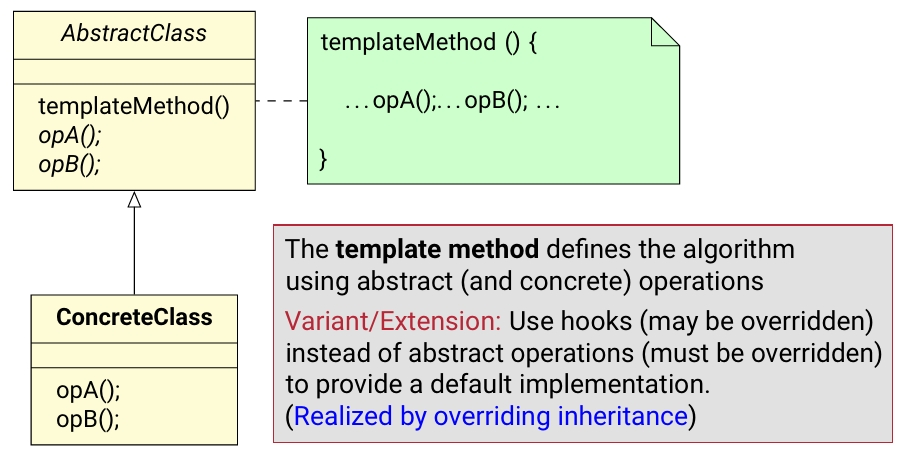
\includegraphics[width=1\textwidth]{Images/The Template Method Pattern.jpeg}
\end{figure}
\begin{defBox}[title=Benefits of the Template Method Pattern]
    \begin{itemize}
        \item \red{Separation} of variant and invariant parts
        \item Avoidance of \red{code duplication} in subclasses (commom behavior is factored out)
        \item Control of subclass \red{extensions}
    \end{itemize}
\end{defBox}

\subsection{Part IV: Design Patterns-General Properties}
\subsubsection{Design Patterns: Benefits \& Essentials}
\blue{Benefits}\\
\red{Systematic} (software) development:
\begin{itemize}
    \item \red{Document} expert knowledge
    \item \red{Reuse} of general and good solutions that worked well before
    \item Raising the \red{abstraction level} of code/documentation
\end{itemize}
\blue{Essentials}
\begin{itemize}
    \item A pattern has a \red{name}
    \item The adressed problem (and its solution) is \red{relevant} (problem occurs regularly, not a one-off problem)
    \item The solution can be easily \red{adapted} to a variant of the problem
\end{itemize}
\begin{defBox}
    A \red{Design Pattern} describes a solution for a problem in a context
\end{defBox}
\subsubsection{Essential Elements of a Software Design Pattern}
\red{Pattern Name} Short mnemonic to extend the design vocabulary\\
\red{Problem Description}
\begin{itemize}
    \item \red{When} to apply the pattern
    \item Conditions under which the pattern provides a \red{solution}
\end{itemize}
\red{Solution}
\begin{itemize}
    \item \red{Elements} constitution the design 
    \item \red{Relationships}, \red{responsibilities}, \red{collaborations} amon these elements
\end{itemize}
\red{Consequences} Trade-offs of applying the pattern, for example:
\begin{itemize}
    \item Language and implementation issues
    \item \red{Impact} on flexibility, extensibility, or portability
\end{itemize}
\subsubsection{Template for a Design Pattern}
\begin{figure}[h]
    \centering
    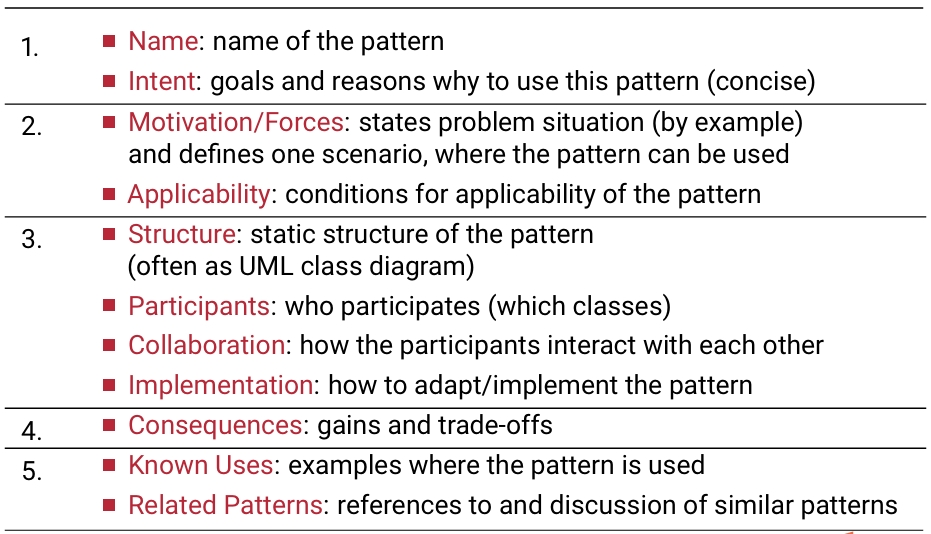
\includegraphics[width=1\textwidth]{Images/Template for a Design Pattern.jpeg}
\end{figure}
\clearpage
\subsubsection{Design Patterns Serve Multiple Purposes}
\begin{figure}[h]
    \centering
    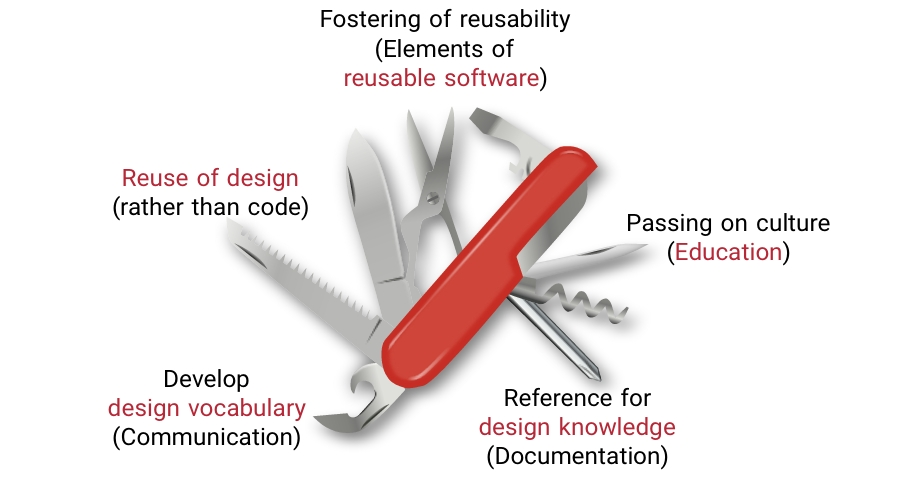
\includegraphics[width=1\textwidth]{Images/Design Patterns Serve Multiple Purposes.jpeg}
\end{figure}
\begin{defBox}
    Patterns aim to enable construcation of high-quality software architectures
\end{defBox}
\begin{defBox}
    Software design patterns describe 
    \begin{itemize}
        \item commonly recurring structures of interacting software components
        \item that solve general design problems within a particular context
    \end{itemize}
\end{defBox}
\subsubsection{Occurrences of Design Patterns Outside Software}
\blue{Some usages of design patterns:}
\begin{itemize}
    \item \red{Chess:} from rules to expertise
    \item \red{Agriculture:} wisdom vs. science
    \item \red{Architecture:} pioneering work on design patterns by \blue{C. Alexander}
\end{itemize}